\subsection{Les capteurs}
Pour exploiter correctement un système automatisé, il est essentiel de \textbf{controler les variations de certaines grandeurs physiques} et \textbf{l'état physique de certains de ses constituants}.

Les capteurs sont des composants permettant d'acquérir une information en provenance du monde extérieur. Dans le cas d'un automate industriel, ils permettent de connaître l'état du système et de mesurer les variations des grandeurs physiques qui lui sont associées.

\UPSTIdefinition{Un capteur transforme une grandeur physique en une grandeur normée, généralement électrique, qui peut être interprétée par un dispositif de contrôle
commande comme l’API.}

\UPSTIaRetenir{Un automate industriel acquiert des informations sur l'état d'un système à l'aide de \textbf{capteurs}}

Il existe trois familles de capteurs se différenciant par la nature du signal qu'ils mesurent :

\begin{description}
	\item [Capteurs Analogiques : ] Le signal délivré est la traduction de la grandeur physique mesurée. Le signal en sortie est généralement sous la forme d'un courant ou d'une tension variable.

	\begin{itemize}
		\item Sonde de température
		\item Capteur de luminosité
		%\item Microphone
		\item Sonde de déformation
		\item \dots
	\end{itemize}

	\item [Capteurs logiques (Tout Ou Rien - TOR) : ] Le signal ne peut prendre que deux valeurs représentant les états 0 et 1. Ces capteurs sont aussi appelés des \textit{détecteurs}.
		\begin{itemize}
			\item Détecteur de proximité
			\item Capteur fin de course de vérin
			\item Détecteur infrarouge
			\item \dots
		\end{itemize}

			\item[Capteurs numériques :] Le signal est codé au sein du capteur. Il est ensuite envoyé sous la forme d'un signal variant de façon discrète dans le temps.
			\begin{itemize}
				\item Codeur d'un moteur
				\item Capteur de température numérique
				\item \dots
			\end{itemize}
\end{description}

La Figure~\ref{fig:analogVsNum} rappelle la forme des signaux analogique et numériques

\begin{figure}[ht]
\centering
\begin{subfigure}{0.49\textwidth}
\centering
	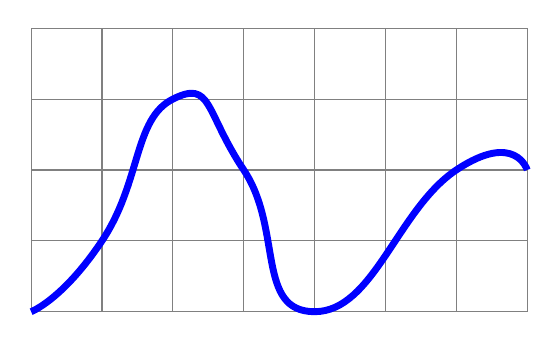
\begin{tikzpicture}[scale = 0.9]
\draw [gray](0,0) grid (7,4);
\draw [blue, line width = 2.5pt] plot [smooth, tension=1] coordinates { (0,0) (1,1) (2,3) (3,2) (4,0) (6,2) (7,2)};
\end{tikzpicture}

	\caption{Signal analogique}
\end{subfigure}%
%
\begin{subfigure}{0.49\textwidth}
\centering
	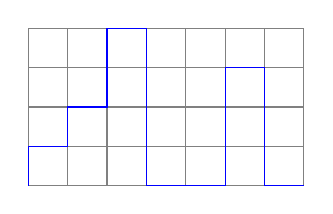
\begin{tikzpicture}[scale = 0.5]
\draw [gray](0,0) grid (7,4);
\draw [blue] plot coordinates { (0,0) (0,1) (1,1) (1,2) (2,2) (2,4) (3,4) (3,0) (5,0) (5,3) (6,3) (6,0) (7,0)};
\end{tikzpicture}

	\caption{Signal numérique}
\end{subfigure}
%
	\caption{Rappel -- signal analogique et numérique}
	\label{fig:analogVsNum}
\end{figure}

\UPSTIremarque[Conversion analogique - numérique]{Il est possible de convertir un signal analogique en un signal numérique. Voir exemple en TD.\\}


\begin{UPSTIactivite}
\UPSTIquestion{De quel type (analogique, numérique ou logique) sont les capteurs inductif et optique ci-dessous ?}

\UPSTIlignesACompleter[1]{logiques (TOR) car ils ne peuvent prendre que deux valeurs : 1 ou 0.}

	 \begin{minipage}[t]{.45\textwidth}
	\begin{center}
		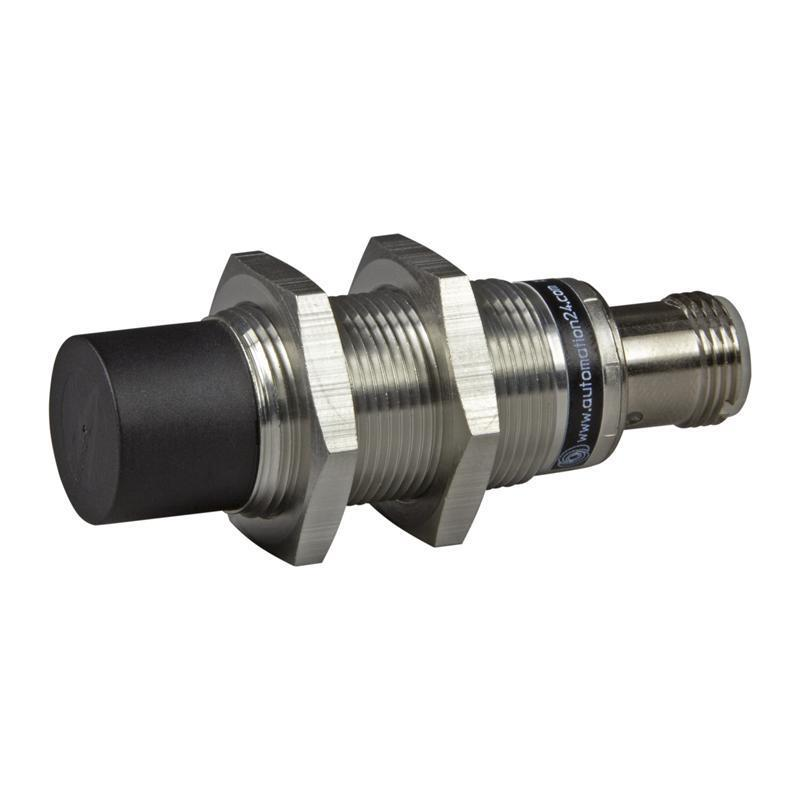
\includegraphics[width=.4\textwidth,height=.4\textheight,keepaspectratio]{images/capt_inductif}
	\end{center}


		Un \textbf{capteur inductif} détecte la présence d'objets métalliques.
	\end{minipage}\hfill
	\begin{minipage}[t]{.45\textwidth}
	\begin{center}
		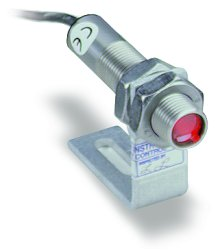
\includegraphics[width=.4\textwidth,height=.3\textheight,keepaspectratio]{images/capt_optique}
	\end{center}
		Un \textbf{capteur optique} détecte la présence d'un objet à l'aide d'un faisceau optique.
	\end{minipage}

	Ces deux capteurs renvoient un signal \textbf{0} ou \textbf{1} selon si un objet est présent à proximité ou non.


	\UPSTIquestion{De quel type (analogique, numérique ou logique) est le codeur optique ci-dessous ?}

	\UPSTIlignesACompleter[1]{Numérique car il donne un signal temporel discret (succession de 0 et de 1).}

		\begin{minipage}[b]{.9\textwidth}
		\begin{center}
			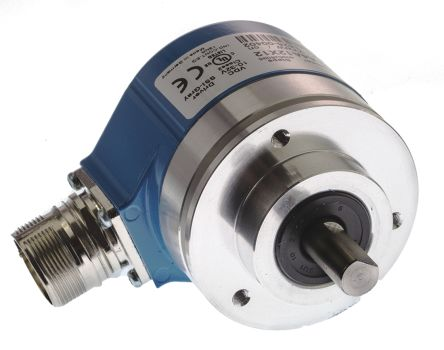
\includegraphics[width=.2\textwidth,height=.3\textheight,keepaspectratio]{images/codeur_optique}
		\end{center}

			Un \textbf{codeur optique} renvoie \textit{un signal carré} dont les caractéristiques permettent de connaitre la position et/ou la vitesse d'un moteur.
		\end{minipage}

		\UPSTIquestion{De quel type (analogique, numérique ou logique) est la sonde de température ci-dessous ?}

		\UPSTIlignesACompleter[1]{Analogique car tension continue image d'une température. }

			\begin{minipage}[b]{.9\textwidth}
			\begin{center}
				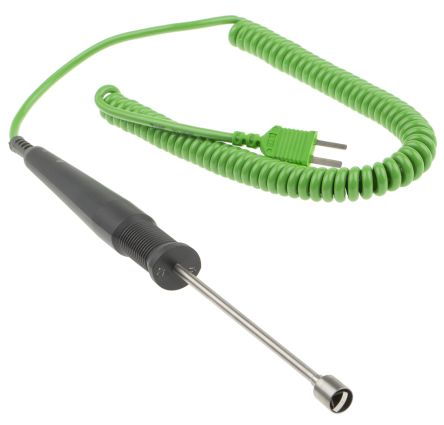
\includegraphics[width=.2\textwidth,height=.3\textheight,keepaspectratio]{images/sondeTemperature}
			\end{center}

				Une \textbf{sonde de température} renvoie \textit{un courant ou une tension} variant de $V_{\text{min}}$ à  $V_{\text{max}}$ en fonction de la température.
			\end{minipage}
\end{UPSTIactivite}
